%!TEX program = xelatex
\documentclass[dvipsnames, svgnames,a4paper,11pt]{article}
% ----------------------------------------------------
%   中山大学物理与天文学院本科实验报告模板
%   作者:Huanyu Shi,2019级
%   知乎:https://www.zhihu.com/people/za-ran-zhu-fu-liu-xing
%   Github:https://github.com/Huanyu-Shi/SYSU-SPA-Labreport-Template
%   Last update : 2023.4.10
% ----------------------------------------------------

% ----------------------------------------------------- 
%	加边框的命令
%	参考:https://tex.stackexchange.com/questions/531559/how-to-add-the-page-border-for-first-two-pages-in-latex
\usepackage{tikz}
\usetikzlibrary{calc}
\usepackage{eso-pic}
\AddToShipoutPictureBG{%
\begin{tikzpicture}[overlay,remember picture]
\draw[line width=0.6pt] % 边框粗细
    ($ (current page.north west) + (0.6cm,-0.6cm) $)
    rectangle
    ($ (current page.south east) + (-0.6cm,0.6cm) $); % 边框位置
\end{tikzpicture}}


\usepackage{xcolor}
\definecolor{c1}{HTML}{2752C9} % 目录颜色
\definecolor{c2}{RGB}{190,20,83} % 引用颜色

\usepackage{ctex}
\usepackage[top=28mm,bottom=28mm,left=15mm,right=15mm]{geometry}
\usepackage{hyperref} 
\hypersetup{
	colorlinks,
	linktoc = section, % 超链接位置,选项有section, page, all
	linkcolor = c1, % linkcolor 目录颜色
	citecolor = c1  % citecolor 引用颜色
}
\usepackage{amsmath,enumerate,multirow,float}
\usepackage{tabularx}
\usepackage{tabu}
\usepackage{subfig}
\usepackage{fancyhdr}
\usepackage{graphicx}
\usepackage{wrapfig}  
\usepackage{physics}
\usepackage{appendix}
\usepackage{amsfonts}

%
\usepackage{tcolorbox}
\tcbuselibrary{skins,breakable}
\newtcolorbox{tbox}[2][]{
    colframe=black!70!,
    breakable,
    enhanced,
	boxrule =0.5pt,
    title = {#2},
    fonttitle = \large\kaishu\bfseries,
	drop fuzzy shadow,
    #1
}
\newtcolorbox[auto counter,number within=section]{question}[1][]{
  top=2pt,bottom=2pt,arc=1mm,
  boxrule=0.5pt,
%   frame hidden,
  breakable,
  enhanced, %跨页后不会显示下边框
  coltitle=c1!80!gray,
  colframe=c1,
  colback=c1!3!white,
  drop fuzzy shadow,
  title={思考题~\thetcbcounter:\quad},
  fonttitle=\bfseries,
  attach title to upper,
  #1
}
\newcommand{\setLhead}[1]{%
  \lhead{{\color{gray}\kaishu #1}} % 定义新的命令,设置右边页眉的内容
}
\newcommand{\setRhead}[1]{%
  \rhead{{\color{gray}\kaishu #1}} % 定义新的命令,设置右边页眉的内容
}
% ---------------------------------------------------------------------
%	利用cleveref改变引用格式,\cref是引用命令
\usepackage{cleveref}
\crefformat{figure}{#2{\textcolor{c2}{图 #1}}#3} % 图片的引用格式
\crefformat{equation}{#2{(\textcolor{c2}{#1})}#3} % 公式的引用格式
\crefformat{table}{#2{\textcolor{c2}{表 #1}}#3} % 表格的引用格式


% ---------------------------------------------------------------------
%	页眉页脚设置
\fancypagestyle{plain}{\pagestyle{fancy}}
\pagestyle{fancy}
\setLhead{中山大学物理与天文学院基础物理实验预习报告}
%\lhead{\kaishu 中山大学物理与天文学院物理实验\uppercase\expandafter{\romannumeral3}} % 左边页眉,学院 + 课程
%\rhead{{\color{gray}\kaishu Template 实验报告模板}} % 右边页眉,实验报告标题
\setRhead{实验1\hspace{1pt}冰的熔化热测量}
\cfoot{\thepage} % 页脚,中间添加页码


% ---------------------------------------------------------------------
%	对目录、章节标题的设置
\renewcommand{\contentsname}{\centerline{\huge 目录}}
\usepackage{titlesec}
\usepackage{titletoc}
% \titleformat{章节}[形状]{格式}{标题序号}{序号与标题间距}{标题前命令}[标题后命令]
\titleformat{\section}{\centering\LARGE\songti}{}{1em}{}

% ---------------------------------------------------------------------
%   listing代码环境设置
\usepackage{listings}
\lstloadlanguages{python}
\lstdefinestyle{pythonstyle}{
backgroundcolor=\color{gray!5},
language=python,
frameround=tftt,
frame=shadowbox, 
keepspaces=true,
breaklines,
columns=spaceflexible,                   
basicstyle=\ttfamily\small, % 基本文本设置,字体为teletype,大小为scriptsize
keywordstyle=[1]\color{c1}\bfseries, 
keywordstyle=[2]\color{Red!70!black},   
stringstyle=\color{Purple},       
showstringspaces=false,
commentstyle=\ttfamily\scriptsize\color{green!40!black},%注释文本设置,字体为sf,大小为smaller
tabsize=2,
morekeywords={as},
morekeywords=[2]{np, plt, sp},
numbers=left, % 代码行数
numberstyle=\it\tiny\color{gray}, % 代码行数的数字字体设置
stepnumber=1,
rulesepcolor=\color{gray!30!white}
}




% ---------------------------------------------------------------------
%	其他设置
\def\degree{${}^{\circ}$} % 角度
\graphicspath{{./images/}} % 插入图片的相对路径
\allowdisplaybreaks[4]  %允许公式跨页 % 导入模板的相关设置
\usepackage{lipsum}
\usepackage{indentfirst}
\usepackage{pdfpages}
\renewcommand{\d}{\mathrm{d}}


%---------------------------------------------------------------------
%	正文
%---------------------------------------------------------------------
\setRhead{实验1\hspace{0.3cm}冰的熔化热测量}%实验名称
\begin{document}


\begin{table}
	\renewcommand\arraystretch{1.7}
	\begin{tabularx}{\textwidth}{
		|X|X|X|X
		|X|X|X|X|}
	\hline
	\multicolumn{2}{|c|}{预习报告}&\multicolumn{2}{|c|}{实验记录}&\multicolumn{2}{|c|}{分析讨论}&\multicolumn{2}{|c|}{总成绩}\\
	\hline
	98& &96 & & & & & \\
	\hline
	\end{tabularx}
\end{table}


\begin{table}
	\renewcommand\arraystretch{1.7}
	\begin{tabularx}{\textwidth}{|X|X|X|X|}
	\hline
	专业:& 物理学类 &年级:& 2023级\\
	\hline
	姓名:& 姚昊廷  & 学号:&22322091\\
	\hline
	实验时间:& 2024.9.19& 教师签名:& \\
	\hline
	\end{tabularx}
\end{table}

\begin{center}
	\LARGE 实验1\hspace{0.3cm}冰的熔化热测量
\end{center}

\textbf{【实验报告注意事项】}
\begin{enumerate}
	\item 实验报告由三部分组成:
	\begin{enumerate}
		\item 预习报告:(提前一周)认真研读\underline{\textbf{实验讲义}},弄清实验原理;实验所需的仪器设备、用具及其使用(强烈建议到实验室预习),完成课前预习思考题;了解实验需要测量的物理量,并根据要求提前准备实验记录表格(第一循环实验已由教师提供模板,可以打印)。预习成绩低于10分(共20分)者不能做实验。
	    \item 实验记录:认真、客观记录实验条件、实验过程中的现象以及数据。实验记录请用珠笔或者钢笔书写并签名(\textcolor{red}{\textbf{用铅笔记录的被认为无效}})。\textcolor{red}{\textbf{保持原始记录,包括写错删除部分,如因误记需要修改记录,必须按规范修改。}}(不得输入电脑打印,但可扫描手记后打印扫描件);离开前请实验教师检查记录并签名。
	    \item 分析讨论:处理实验原始数据(学习仪器使用类型的实验除外),对数据的可靠性和合理性进行分析;按规范呈现数据和结果(图、表),包括数据、图表按顺序编号及其引用;分析物理现象(含回答实验思考题,写出问题思考过程,必要时按规范引用数据);最后得出结论。
	\end{enumerate}
	\textbf{实验报告就是将预习报告、实验记录、和数据处理与分析合起来,加上本页封面。}
	\item 每次完成实验后的一周内交\textbf{实验报告}(特殊情况不能超过两周)。
	\item 除实验记录外,实验报告其他部分建议双面打印。
\end{enumerate}

{\color{red}\textbf{【实验安全与实验室注意事项】}
\begin{enumerate}
	\item 使用热水和冰块注意避免烫伤、冻伤。
	\item 运输水时,注意他人的安全,避免把水弄到地上。
\end{enumerate}}

\clearpage
\tableofcontents
\clearpage

\setcounter{section}{0}
\section{实验1\hspace{0.3cm}冰的熔化热测量}
	
\subsection{实验目的}
\begin{enumerate}
	\item 掌握混合法测量冰的熔化热基本原理,学习物理建模;
	\item 测定冰的熔化热。
\end{enumerate}

\subsection{仪器用具}
\begin{table}[htbp]
	\centering
	\renewcommand\arraystretch{1.6}
	% \setlength{\tabcolsep}{10mm}
	\begin{tabular}{p{0.05\textwidth}|p{0.20\textwidth}|p{0.05\textwidth}|p{0.5\textwidth}}
	\hline
	编号& 仪器用具名称 & 数量 &  主要参数(型号,测量范围,测量精度等) \\
	\hline
	1&MS6514测温仪 &2 & 配两对K型热电偶\\

	2&保温杯 &1& \\
	
	3&量杯 & 1 &350mL或500mL \\
	
	4&电子天平&1 & 量程1000g,最小分辨率0.01g\\
	\hline
\end{tabular}
\end{table}

\subsection{原理概述}
\begin{question}
	一、简述热力学第一定律。
\tcblower
物体内能的增加等于物体吸收热量与外界对物体做功之和,用数学语言表示为
$$\Delta U=Q+W$$
\end{question}
\begin{question}
	二、简述利用混合法来测定冰的熔化热的原理,列出必要的公式。
	\tcblower
	在一定压强下,固体发生熔化时的温度称为熔化温度或熔点,单位质量的固态物质在熔
点时完全熔化为同温度的液态物质所需要吸收的热量称为熔化热,用 $L$ 表示,单位为 J/kg
或 J/g。
将质量为$m$、温度为$0^\circ$C的冰块置入量热器内,与质量为$m_0$、温度为$T_0$的水相混合,设量
热器内系统达到热平衡时温度为$T_1$。若忽略量热器与外界的热交换,即将水、冰和量热器看作是孤立系统,根据热平衡原理可知,冰块熔化成水并升温吸热与水和量热器内筒的降温放
热相等:
$$mL+mC_0(T_1-T')=(m_0C_0+m_1C_1)(T_0-T_1) $$
式中,$T_0,T_1$分别 为投冰前、后水的近平衡温度,
$T'$为冰的熔点 ($0^\circ$C),$m$为冰的质量,$m_0$为量热器内筒中所取温水的质量;
$C_0=4.18J/(g\cdot^\circ C)$为水的比热; $m_1$为量热器内筒质量、 $C_1$为量热器内筒比热 。
\end{question}


\subsection{实验前思考题}
\begin{question}
	(4-1)式的建立(建模)做了哪些简化?
	\tcblower
	\begin{enumerate}
		\item 忽略容器与外界热交换,即将水冰和量热器视作孤立系统。
		\item 忽略搅拌器所做的功对系统造成的内能升高。
		\item 忽略水在该过程中的蒸发。
		\item 忽略容器中空气温度变化。
		\item 认为容器热容稳定且始终温度均匀。
		\item 假定水的比热容恒定。
	\end{enumerate}
\end{question}

\begin{question}
	保温杯$m_1C_1$估算所基于的模型作了什么简化?请分析其误差(选)
	\tcblower
	\begin{enumerate}
		\item 忽略未与水直接接触的内壁部分。
		\item 忽略内外胆之间的热辐射。
		\item 假定不锈钢热容稳定。
		\item 忽略保温杯内部细节。
	\end{enumerate}
	在实验中保温杯上部温度低于下部温度会导致测量值比实际值偏小。
\end{question}

\begin{question}
	(可通过实验回答)不用搅拌器对冰的熔化时间延长多久,对测量精度由多大的影响?
	\tcblower
	在实验2中不用搅拌器会使冰的熔化时间延长5-6秒,使得吸热增多,测量出的熔化热值偏小。
	但是由于温差不大以及时间不长,导致对实验精度影响不大。
\end{question}

\begin{question}
	(选)外推法修正漏热的物理原理是什么?能否推导出来?
	\tcblower
	\begin{figure}[H]
		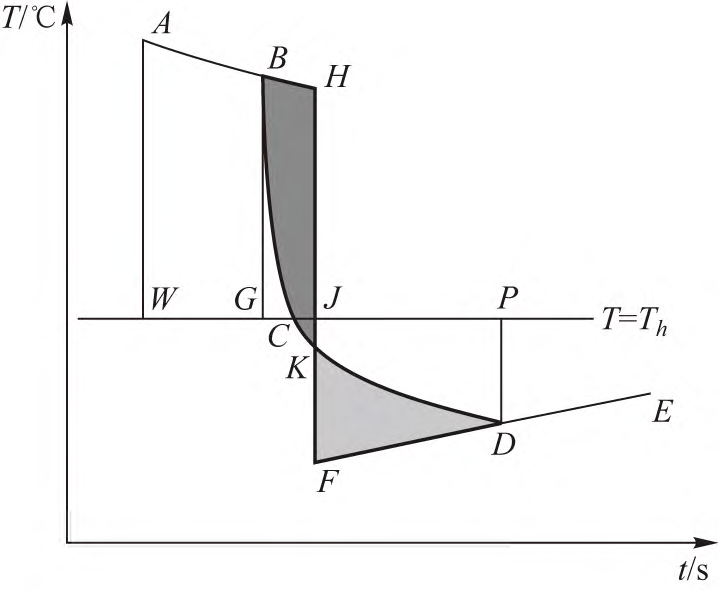
\includegraphics[width=0.5\textwidth]{yuxi.png}
	\end{figure}
	对于热容为$C$、温度为$T$的均匀热系统,其总热量的$Q$变化率等于热容乘以系统温度的变化率,即
$$\frac{\d Q}{\d t}=C\frac{\d T}{\d t}$$
在$T-t $图的AB 段,系统的$C = C_S$,系统热量变化主要由自然对流引起,设对流交换的热量为$Q_1$,则
$\d Q= \d Q_1$ 。 在系统温度与环境温差$( T-T_h) $
较小的情况下,由牛顿冷却定律有
$$\frac{\d Q_1}{\d t}=K(T-T_h)$$
其中,$K$ 为系统在空气中的对流散热系数. 联立公式右侧构成微分方程,对其分离变量并积
分,可以得到温度随时间变化的解析表达式为
$$T-T_h=(T_A-T_h)e^{(K/C_s)(t-t_A)}$$
其中,$( t_A,T_A) $是图1 中A 点的坐标. 但由于$(K/C_s)(t-t_A)$
很小,又可以将其 近似表示为线性函数.则有
$$T\approx (K/C_S)(T_A-T_h)(t-t_A)+T_A$$
假设H 处于自然降温曲线AB 的延长线上,联立公
式的右侧建立等式,并在等号两侧分别乘
以$dt$,对BH 段温度和时间分别积分则有
$$T_H-T_B=(K/C_S)\int_{t_B}^{t_H}(T-T_h)\d t=(K/C_S)S_{BHJG}$$
假设整个实验过程中室温$T_h$不变,且系统a 与混合系统的表面积也不变,所以对流传热系数$K$ 不
变. 在冰熔解完的DE 阶段,$\d Q = \d Q1$
,$C = C'_S = C_S +M_c$. 类比上面公式的分析过程,推导后可得
$$\begin{aligned}
	T-T_h&=(T_D-T_h)e^{(K/C'_S)(t-t_D)}\\
	T&\approx (K/C'_S)(T_D-T_h)(t-t_D)+T_D
\end{aligned}$$
若F 处于自然升温曲线上,则有
$$T_F-T_D=-(K/C'_S)S_{PDFJ}$$
由于
$$\Delta Q_1=K\int_{t_B}^{t_D}(T-T_h)\d t=KS$$
由图1 可知$S=\int_{t_B}^{t_D}(T-T_h)\d t=S_{BGC}-S_{CPD}$
,即图中BGC 与CPD 所围面积之差。
若HF 连线垂直于t 轴并且使$S_{BHK}=S_{KFD}$,则有
$$S=S_{BGC}-S_{CPD}=S_{BHJG}-S_{PDFJ}$$
可以证明,无论$T-t$曲线与$T = T_h$
的相对位置如何变
化,上式所描述的几何关系总是成立。
由此就可以得到
$$L=C_S(T_H-T_F)/M-cT_F$$
\end{question}

\begin{question}
	如何判断冰的温度为$0^{\circ}C$?
	\tcblower
	观察冰的状态,在一个大气压下冰的熔点十分接近$0^\circ$C,此时冰和水处于共存态
	若观察到冰开始熔化或冰周围出现液态水则证明此时冰已十分接近$0^\circ$C。
\end{question}


\clearpage
\setLhead{中山大学物理与天文学院基础物理实验记录}
\begin{table}
	\renewcommand\arraystretch{1.7}
	\centering
	\begin{tabularx}{\textwidth}{|X|X|X|X|}
	\hline
	专业:& 物理学类 &年级:& 2023级 \\
	\hline
	学号:&22322091 & & \\
	\hline
	姓名:& 姚昊廷 &实验地点:&A515\ E4\\
	\hline
	学生签名:& & 评分: &\\
	\hline
	实验时间:& 2024.9.19& 教师签名:&\\
	\hline
	\end{tabularx}
\end{table}

\section{实验1\hspace{0.3cm}冰的熔化热测量}
\subsection{实验内容}
使用混合法,对已知质量、比热的系统,加入已知质量的冰,测量前后的温度,计算冰的熔化热。
\subsection{实验步骤、结果}
\subsubsection{实验内容1.1}
\begin{table}[!h]
	\renewcommand\arraystretch{1.7}
	\centering
	\begin{tabularx}{\textwidth}{|X|X|X|X|X|X|}
	\hline
	测量次序& $m_c/$g &$m_c+m_0/$g& $m_c+m_0+m/$g&$T_0/^\circ$C&$T_1/^\circ$C \\
	\hline
	1&276.00&709.55&737.08&56.1&47.6\\
	\hline
	2&276.79&690.38&810.54&61.0&55.1\\
	\hline
	\end{tabularx}
\end{table}
\subsubsection{实验内容1.2}
{\bf 冰块熔化前后水温随时间的变化:}(室温$T=25^\circ$C)
\begin{table}[!h]
	\renewcommand\arraystretch{1.7}
	\centering
	\begin{tabularx}{\textwidth}{|X|X|X|X|X|X|}
	\hline
	测量次序& $m_c/$g &$m_c+m_0/$g& $m_c+m_0+m/$g&$m_0/$g&$m/$g \\
	\hline
	1&276.28&685.32&777.54&409.04&92.22\\
	\hline
	2&276.54&685.51&777.59&408.97&92.08\\
	\hline
	3&276.68&685.25&779.84&408.57&94.59\\
	\hline
	\end{tabularx}
\end{table}\par
{\bf 冰块熔化前后水温随时间的变化:}(室温$T=25^\circ$C)
\begin{table}[!h]
    \centering
    \begin{tabular}{|l|l|l|l|l|l|l|l|l|l|l|}
    \hline
        时间/s & 0 & 10 & 20 & 30 & 40 & 50 & 60 & 70 & 80 & 90 \\ \hline
        温度/$^\circ$C& 48.1 & 48.1 & 48.1 & 48.1 & 48.1 & 48.1 & 48.1 & 48.1 & 48.1 & 48.1 \\ \hline
        时间/s & 100 & 110 & 120 & 130 & 140 & 150 & 160 & 170 & 180 & 190 \\ \hline
        温度/$^\circ$C & 48.1 & 48.1 & 48.1 & 48.1 & 48.1 & 48.1 & 48.1 & 48.1 & 48.1 & 48.1 \\ \hline
        时间/s & 200 & 210 & 220 & 230 & 240 & 250 & 260 & 270 & 280 & 290 \\ \hline
        温度/$^\circ$C & 48.1 & 48.1 & 48.1 & 48.1 & 48 & 48 & 48 & 48 & 48 & 48 \\ \hline
        时间/s & 300 & 310 & 320 & 330 & 340 & 350 & 360 & 370 & 380 & 390 \\ \hline
        温度/$^\circ$C & 48 & 48 & 48 & 48 & 48 & 48 & 48 & 48 & 48 & 48 \\ \hline
        时间/s & 400 & 410 & 420 & 430 & 440 & 450 & 460 & 470 & 480 & 490 \\ \hline
        温度/$^\circ$C & 48 & 48 & 48 & 48 & 48 & 48 & 47.2 & 44 & 35.1 & 32.1 \\ \hline
        时间/s & 500 & 510 & 520 & 530 & 540 & 550 & 560 & 570 & 580 & 590 \\ \hline
        温度/$^\circ$C & 30.6 & 29.7 & 29.6 & 28.5 & 27.2 & 26.4 & 26.1 & 26.1 & 25.7 & 25.5 \\ \hline
        时间/s & 600 & 610 & 620 & 630 & 640 & 650 & 660 & 670 & 680 & 690 \\ \hline
        温度/$^\circ$C & 25.2 & 25.1 & 25.1 & 25.2 & 25.2 & 25.2 & 25.2 & 25.2 & 25.2 & 25.2 \\ \hline
        时间/s & 700 & 710 & ~ & ~ & ~ & ~ & ~ & ~ & ~ & ~ \\ \hline
        温度/$^\circ$C & 25.2 & 25.3 & ~ & ~ & ~ & ~ & ~ & ~ & ~ & ~ \\ \hline
    \end{tabular}
\end{table}
\subsubsection{实验内容2}
{\bf 冰块熔化前后水温随时间的变化:}(室温$T=25^\circ$C)
\begin{table}[!h]
	\renewcommand\arraystretch{1.7}
	\centering
	\begin{tabularx}{\textwidth}{|X|X|X|X|X|X|}
	\hline
	测量次序& $m_c/$g &$m_c+m_0/$g& $m_c+m_0+m/$g&$m_0/$g&$m/$g \\
	\hline
	1&30.25&128.33&144.08&98.08&15.75\\
	\hline
	2&30.37&128.98&144.28&98.61&15.30\\
	\hline
	3&30.34&129.18&146.10&98.84&16.92\\
	\hline
	\end{tabularx}
\end{table}\par
{\bf 冰块熔化前后水温随时间的变化:}(室温$T=25^\circ$C)
\begin{table}[!h]
    \centering
    \begin{tabular}{|l|l|l|l|l|l|l|l|l|l|l|}
    \hline
	时间/s & 0 & 10 & 20 & 30 & 40 & 50 & 60 & 70 & 80 & 90 \\ \hline
	温度/$^\circ$C & 38.1 & 37.9 & 37.8 & 37.7 & 37.7 & 37.7 & 37.6 & 37.6 & 37.6 & 37.5 \\ \hline
		时间/s & 100 & 110 & 120 & 130 & 140 & 150 & 160 & 170 & 180 & 190 \\ \hline
        温度/$^\circ$C & 24.9 & 22.9 & 21.9 & 26.2 & 27.6 & 24.4 & 27.4 & 25.4 & 23.4 & 24 \\ \hline
		时间/s & 200 & 210 & 220 & 230 & 240 & 250 & 260 & 270 & 280 & 290 \\ \hline
		温度/$^\circ$C & 23.6 & 23.2 & 23 & 22.9 & 22.9 & 22.8 & 22.9 & 22.9 & 22.9 & 23 \\ \hline
		时间/s& 300 & 310 & 320 & 330 & 340 & 350 & 360 & 370 & 380 & 390 \\ \hline
        温度/$^\circ$C & 23 & 23 & 23 & 23 & 23 & 23 & 23 & 23 & 23 & 23 \\ \hline
		时间/s & 400 & 410 & 420 & 430 & 440 & 450 & 460 & 470 & 480 & 490 \\ \hline
        温度/$^\circ$C & 23 & 23 & 23 & 23 & 23 & 23 & 23 & 23 & 23 & 23 \\ \hline
		时间/s& 500 & ~ & ~ & ~ & ~ & ~ & ~ & ~ & ~ & ~ \\ \hline
        温度/$^\circ$C & 23 & ~ & ~ & ~ & ~ & ~ & ~ & ~ & ~ & ~ \\ \hline
    \end{tabular}
\end{table}\newpage
\subsection{实验过程中遇到的问题记录}
加冰块时测温头需拿出杯中,导致数据记录不准确。冰块浮在表面导致水的温度不均匀。


\clearpage
\setLhead{中山大学物理与天文学院基础物理实验分析与讨论}
\begin{table}
	\renewcommand\arraystretch{1.7}
	\begin{tabularx}{\textwidth}{|X|X|X|X|}
	\hline
	专业:& 物理学 &年级:& 2023级\\
	\hline
	姓名: &姚昊廷 & 学号:& 22322091\\
	\hline
    日期:&2024.9.19 & 评分: &\\
	\hline
	\end{tabularx}
\end{table}

\section{实验1\hspace{0.3cm}冰的熔化热测量 分析与讨论}
\subsection{数据处理分析、分析与讨论}
(多方案并行,可增加相应的分析与讨论的内容)\par
1.水冰质量计算\\
\begin{enumerate}
	\item $m_0=0.70955kg-0.27600kg=0.43355kg;m=0.73708kg-0.70955kg=0.02753kg$
	\item $m_0=0.69038kg-0.27679kg=0.41359kg;m=0.71054kg-0.69038kg=0.02016kg$
	\item $m_0=0.68532kg-0.27628kg=0.40903kg;m=0.77754kg-0.68532kg=0.09222kg$
	\item $m_0=0.68551kg-0.27654kg=0.40897kg;m=0.77759kg-0.68551kg=0.09208kg$
	\item $m_0=0.68525kg-0.27668kg=0.40857kg;m=0.77984kg-0.68525kg=0.09459kg$
	\item $m_0=0.12833kg-0.03025kg=0.09808kg;m=0.14408kg-0.12833kg=0.01575kg$
	\item $m_0=0.12898kg-0.03037kg=0.09861kg;m=0.14428kg-0.12898kg=0.01530kg$
	\item $m_0=0.12918kg-0.03034kg=0.09884kg;m=0.14610kg-0.12918kg=0.01692kg$
\end{enumerate}\newpage
2.潜热计算
\begin{table}[!h]
	\renewcommand\arraystretch{1.7}
	\centering
	\begin{tabularx}{\textwidth}{|X|X|X|X|X|}
	\hline
	测量次序& $m_0/$g &$m/$g& $m_1/$g&$L$(J/g) \\
	\hline
	1&433.55&27.53&138&380.168\\
	\hline
	2&413.59&20.16&138.39&467.872\\
	\hline
	3&409.03&92.22&138.14&337.765\\
	\hline
	4&408.79&92.08&138.27&340.417\\
	\hline
	5&408.57&94.59&138.34&343.943\\
	\hline
	6&98.08&15.75&30.25&300.326\\
	\hline
	7&98.61&15.3&30.37&305.374\\
	\hline
	8&98.84&16.92&30.34&308.852\\
	\hline
	\end{tabularx}
\end{table}\newpage
3.(仅针对实验2)根据上述第5步至第7步所记录的数据,在二维直角坐标纸上作出对应的温度时间曲线,
并作出B点(投冰)、G点(温度回升点)对应的温度值分别为$T_0$和$T_1$。
\begin{figure}[htbp]
	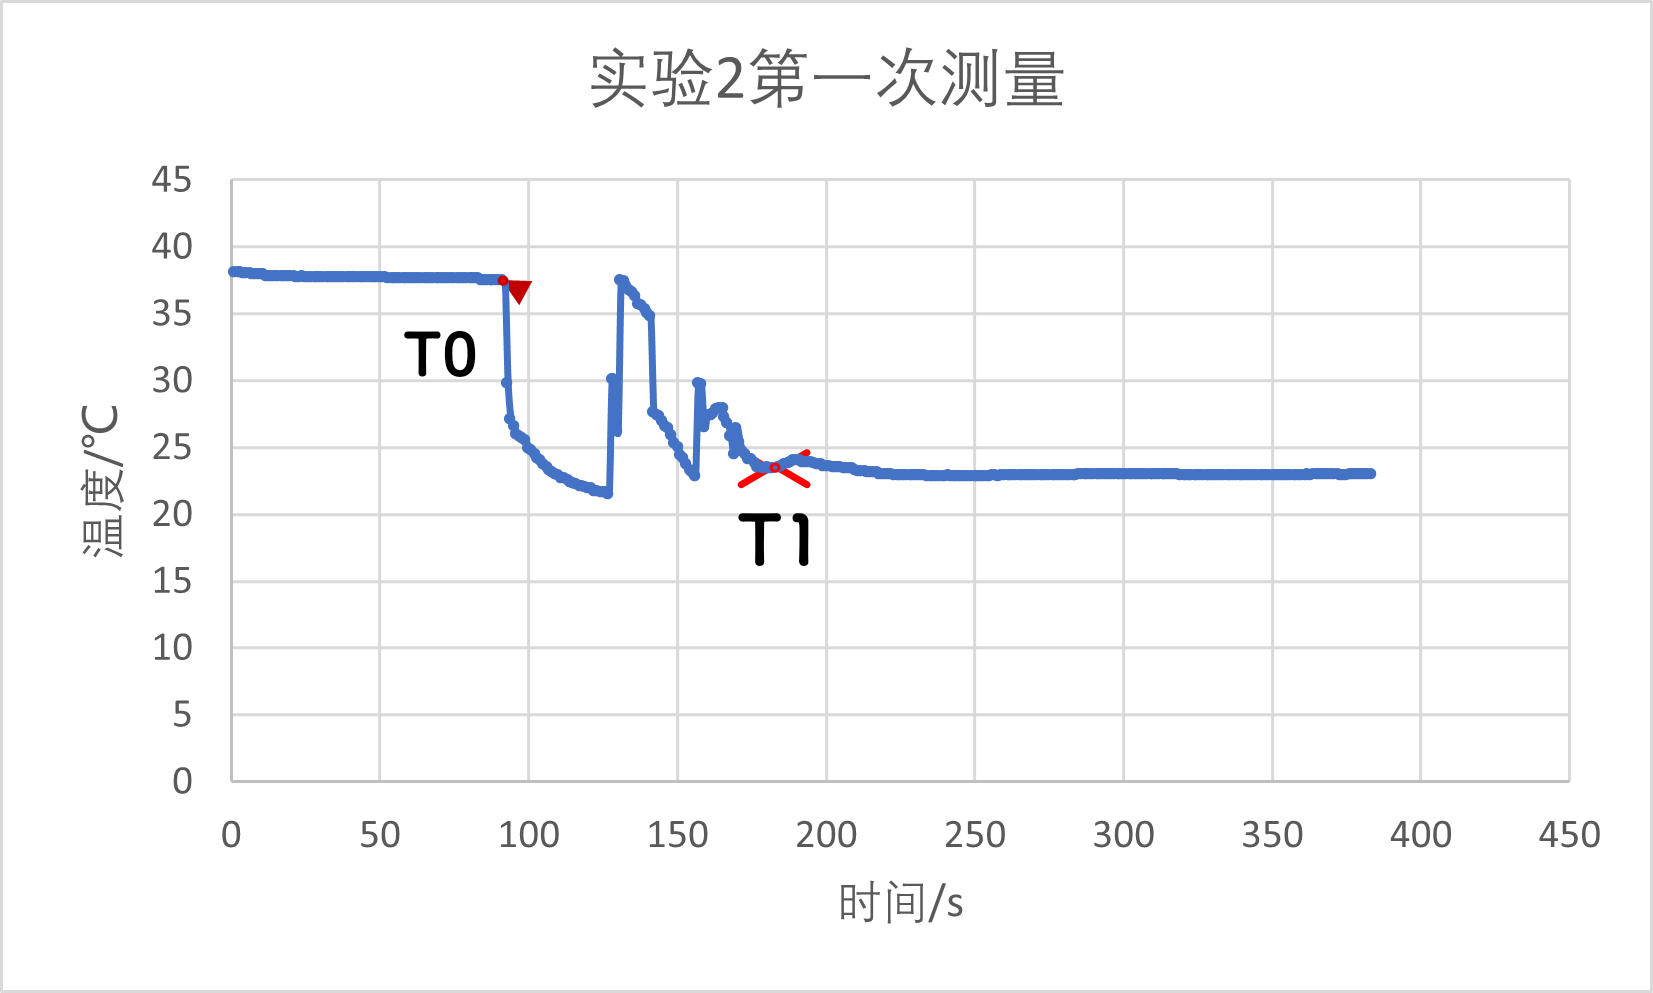
\includegraphics[width=0.95\textwidth]{图片1.png}
\end{figure}
\begin{figure}[htbp]
	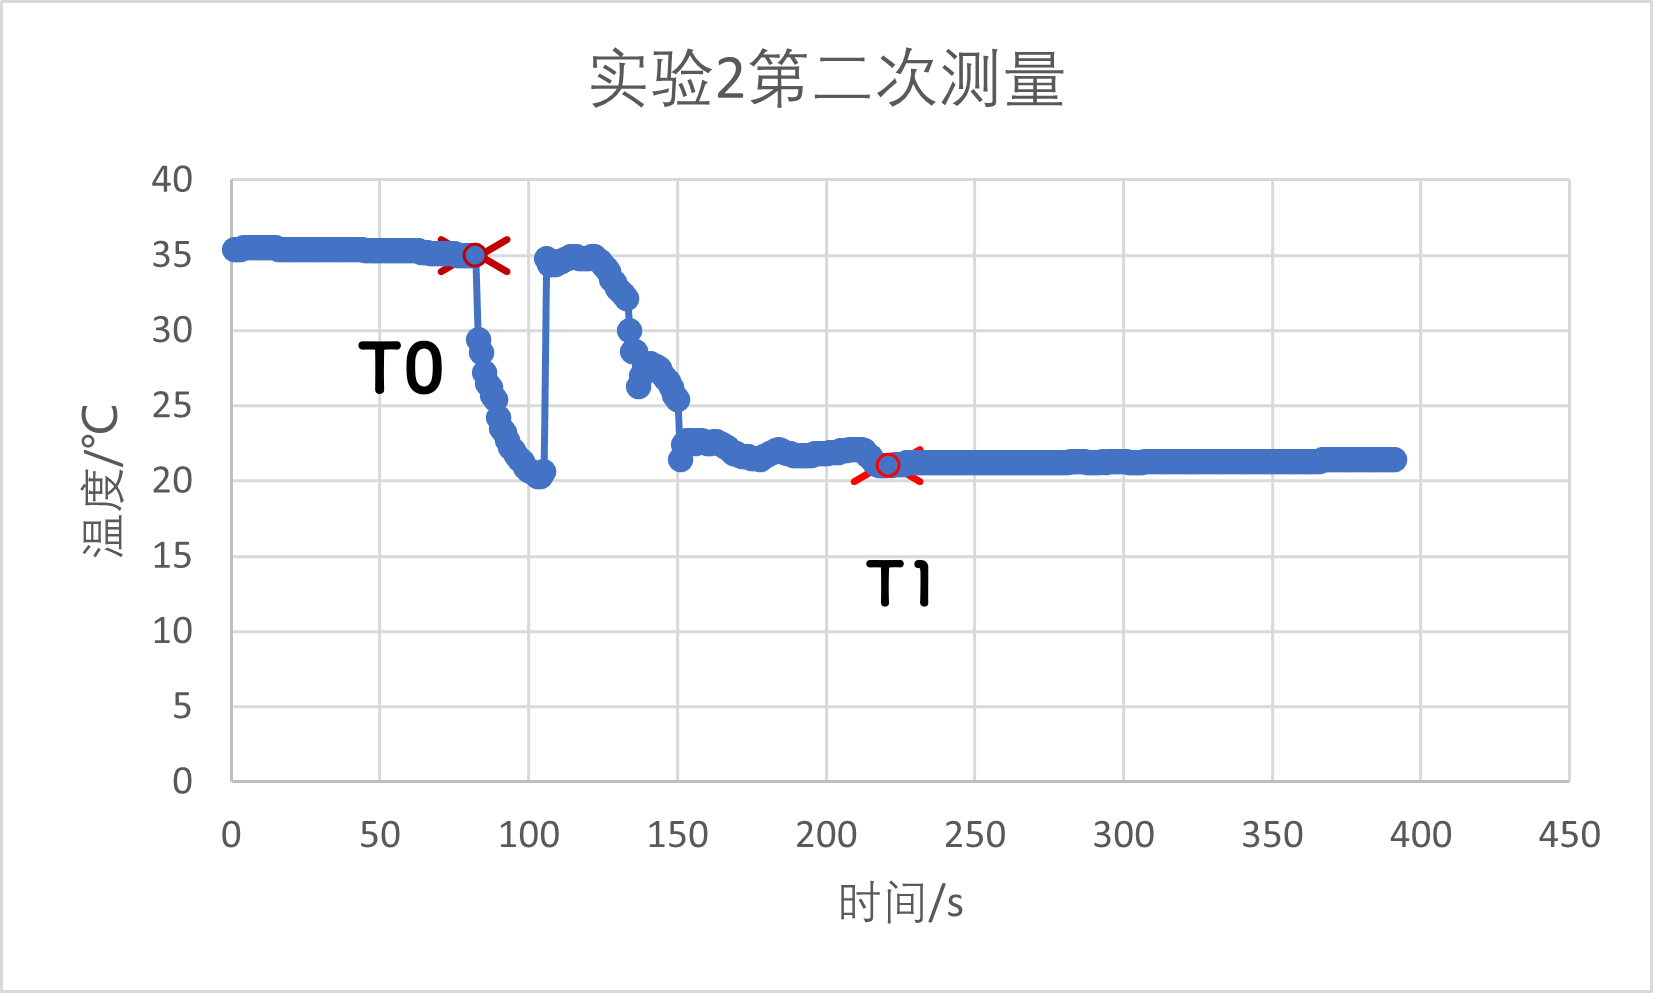
\includegraphics[width=0.95\textwidth]{图片2.png}
\end{figure}
\begin{figure}[!h]
	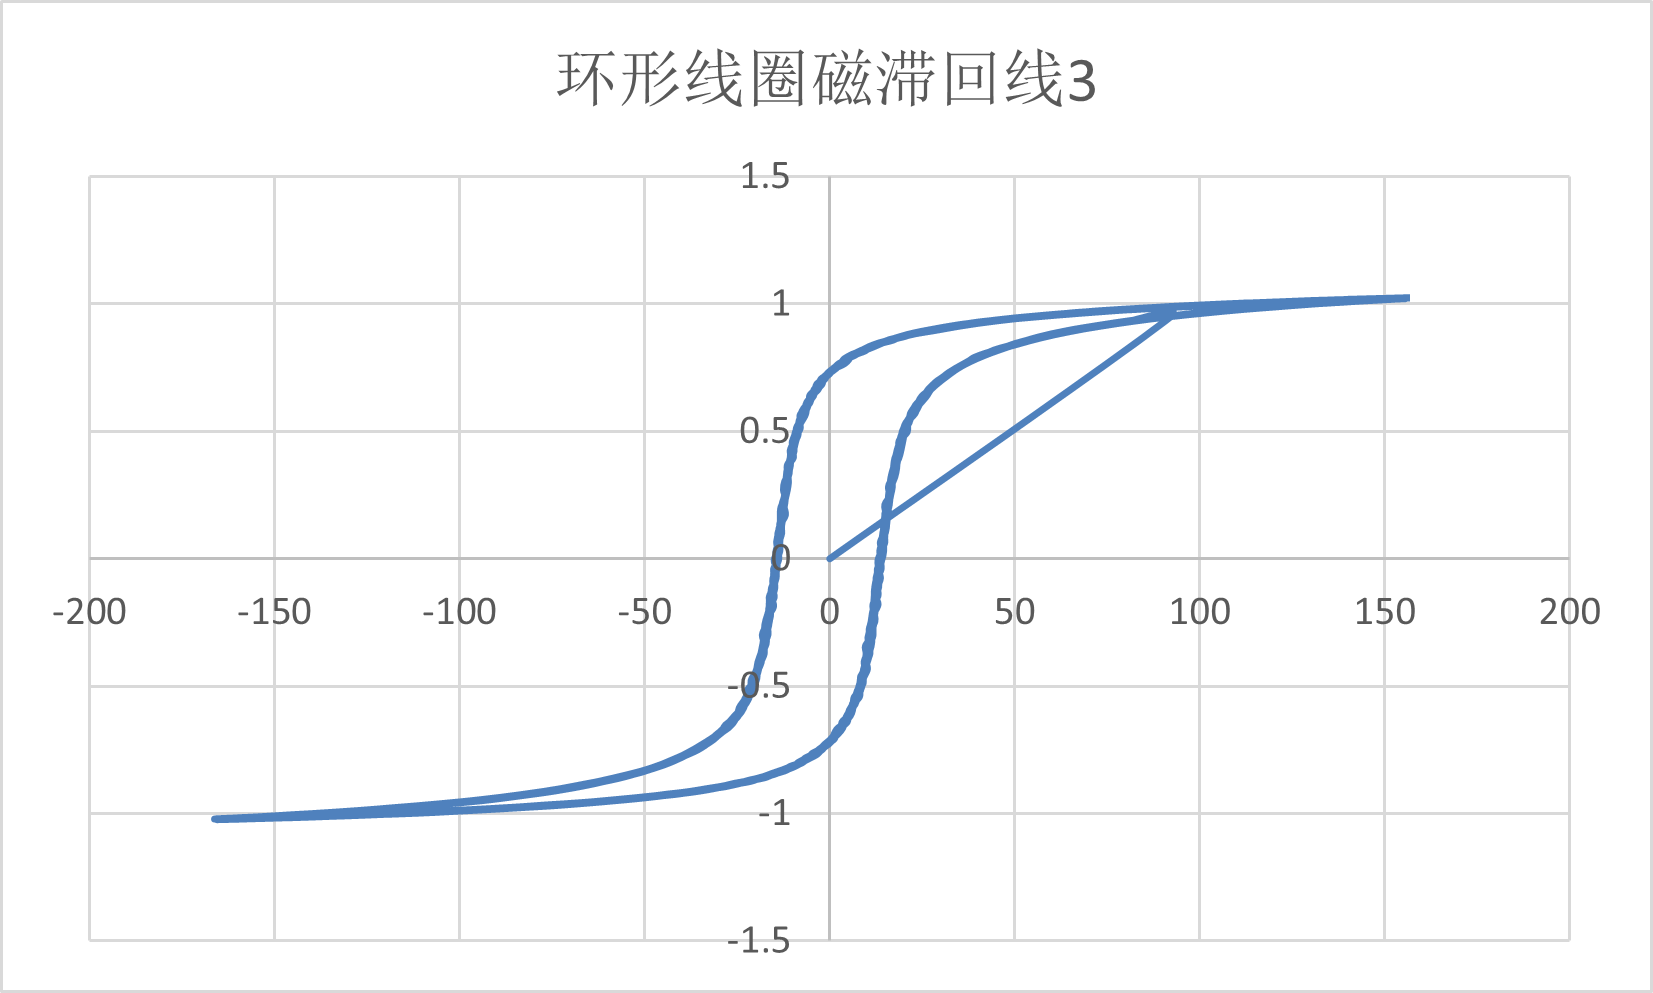
\includegraphics[width=0.95\textwidth]{图片3.png}
\end{figure}\newpage
4.求出冰的熔化热与标准值334J/g相比较;(建议做实验内容1的同学与选实验内容2的同学的数据共享
,比较两种不同实验方案的冰的熔化热测量值)。\\
实验1-1中测出的熔化热明显偏大,1-2较为接近真实值,但仍然偏大,实验2中测量的熔化热均偏小。\par
\vspace{1cm}
5.给出相对误差,并分析误差来源;\\
\begin{table}[!h]
    \centering
    \begin{tabular}{|l|l|l|l|l|l|l|l|l|}
    \hline
	测量次序&1&2&3&4&5&6&7&8\\
	\hline
	L(J/g)&380.168&467.872&337.765&340.417&343.943&300.326&305.374&308.852\\
	\hline
	相对误差&13.8228\%&40.0814\%&1.12725\%&1.92126\%&2.97695\%&10.082\%&8.57066\%&7.52934\%\\
	\hline
    \end{tabular}
\end{table}\\
实验1-1中测出的熔化热明显偏大,因为在摇晃过程中部分水溅到杯盖上,导致水向外界漏热增多,同时部分热量被
杯盖吸收。\\
实验1-2中熔化热测量值,略微偏大。可能是因为实验过程中保温杯漏热导致。\\
实验2中测得熔化热略微偏小,可能是因为冰块放置过久,其内部已经熔化。同时搅拌器加快了熔化速度
使得漏热变少。\par
\vspace{1cm}
6.提出改进办法\\
\begin{enumerate}
	\item 提高保温杯保温效果。
	\item 对保温杯结构进行更细致分析。
	\item 使用搅拌器加快冰的熔化时间。
	\item 选用新鲜冰块,确保冰块温度为$0^\circ$C。
	\item 改进实验装置,使得不用拿出测温仪和打开盖子就可以加入冰块。
	\item 改善实验方法,使得测量质量时不用分次加入冰块。
\end{enumerate}

\subsection{实验后思考题}
\begin{question}
	往量热器内投入冰块后,冰块浮在水面,量热器内温度不均匀,对实验有何影响?(针对所采用实验方案进行讨论。)
	\tcblower
	\begin{enumerate}
		\item 部分冰块直接与空气接触,吸收空气中热量导致测得熔化热偏小。
		\item 冰块与高温水接触面积变小,导致熔化时间变长,使得漏热时间变长。
		\item 冰块与水不完全接触,可能导致冰块还未熔化完全时就已经观测到底部水温上升。
	\end{enumerate}
\end{question}

\begin{question}
	除搅拌外,如何进一步减少这一影响
	\tcblower
	\begin{enumerate}
		\item 升高水温,使得冰块熔化时间变短。
		\item 选用比热容小密度大的物体使冰块沉底。
		\item 换用凹字形容器,使冰块无法浮在水面。
		\item 在水中不同位置放置多个温度计测量不同位置温度减少误差。
	\end{enumerate}
\end{question}

\clearpage
% ---------------------------------------------------------------------
%   参考文献
%   注:使用参考文献时应按照xelatex->bibtex->xelatex->xelatex顺序进行编译
\phantomsection
%\addcontentsline{toc}{section}{参考文献}
\bibliographystyle{unsrt}
\bibliography{myref}
\begin{thebibliography}{9}
	\bibitem{ref1} 凤飞龙,黄育红,金蔚,王公正,崔致远,“外推法计算冰的熔解热的理论依据及Matlab实现方案”,《大学物理》,第42卷,第2期
\end{thebibliography}


\clearpage
\appendix
\appendixpage
\addappheadtotoc
\subsection*{原件扫描}
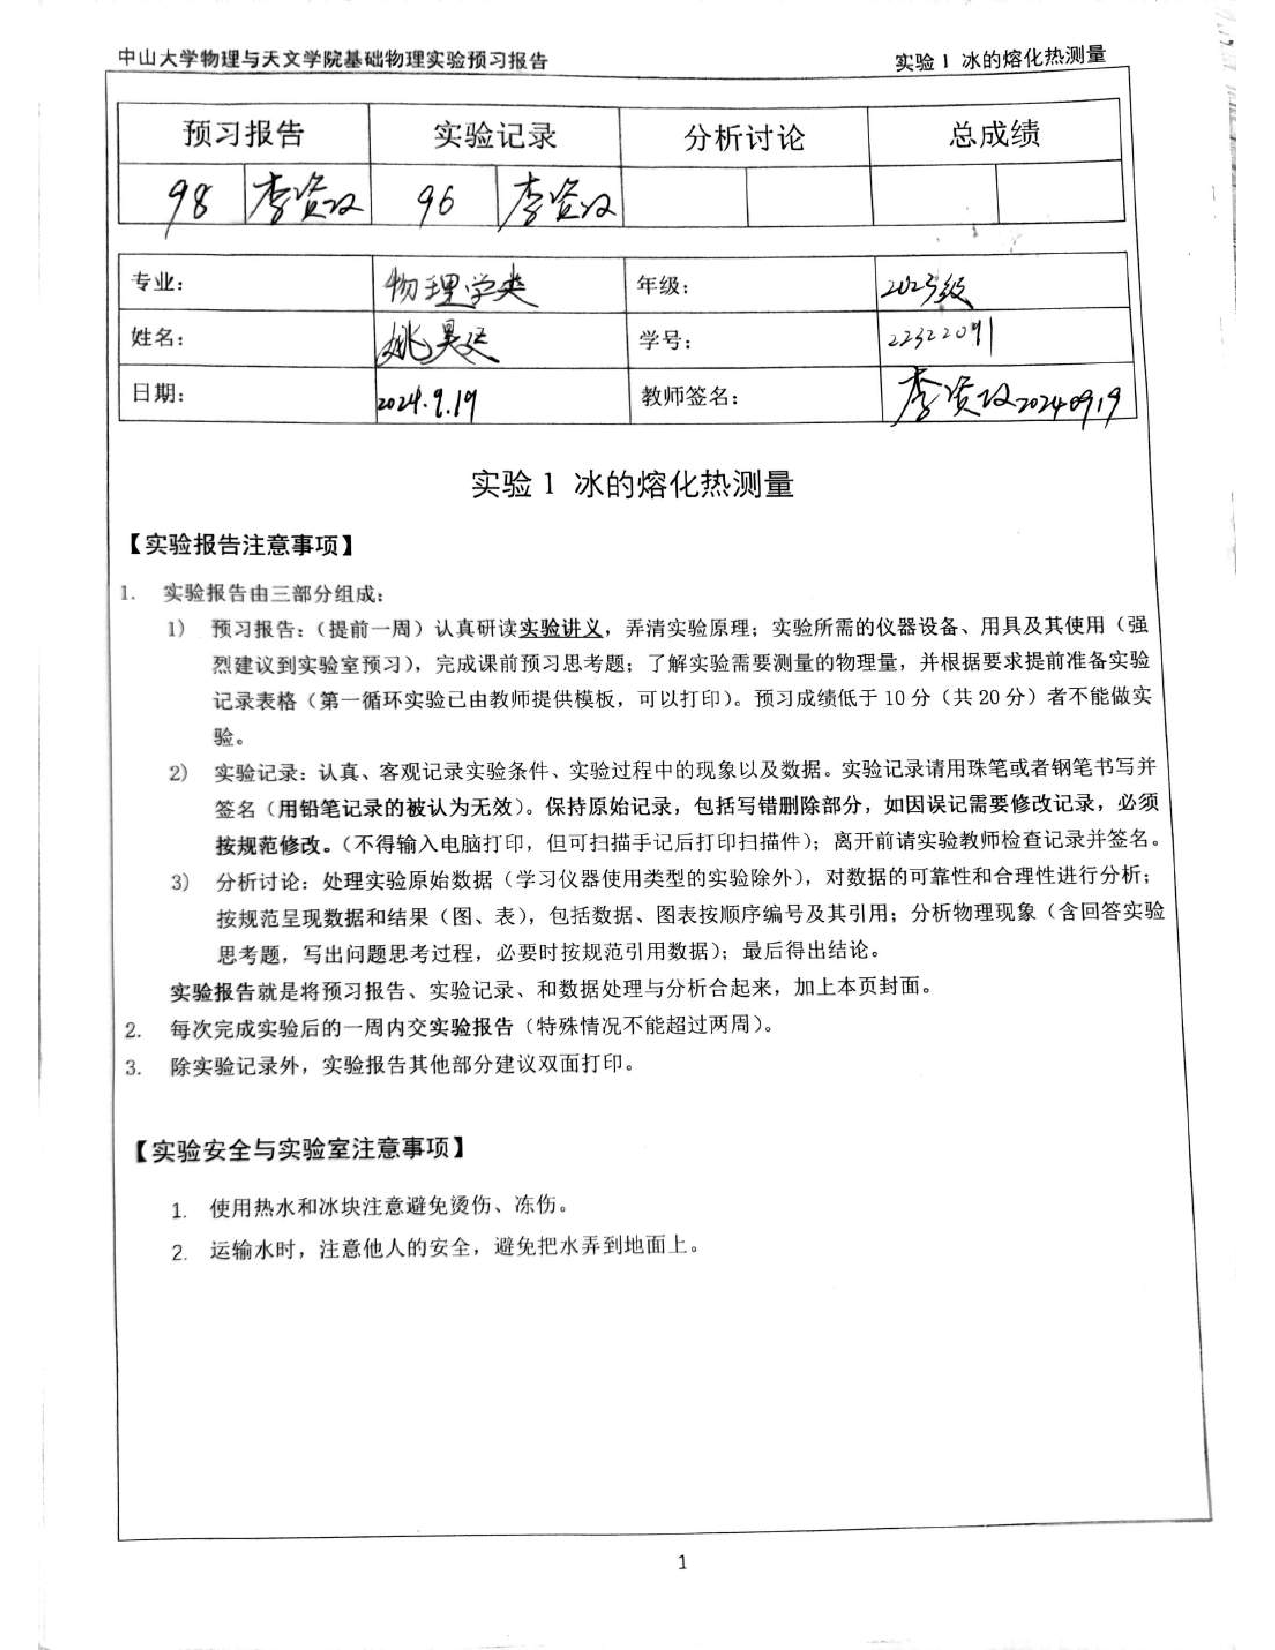
\includepdf[pages=-]{冰扫描件.pdf}
\end{document}

